\section{Secure Distance Measurement}

\paragraph{Introduction} \mbox{} \\
\underline{Applications:}
Wireless car keys, contact tracing in a pandemic, autonomous cars.
\\
\underline{Attacks:}
\textbf{Replay attacks} are an issue, allowing an attacker to make devices appear physically closer (e.g. if the device naively use the observed signal strength to derive the distance).
\\
\underline{Goals:}
(Provably) secure ranging, protecting against all logical and physical attacks and all attacker abilities.
Focus on preventing distance reduction.

\paragraph{Current techniques (overview)} \mbox{} \\
Non-Time-of-Flight:
\begin{itemize}
	\item Received Signal Strength Indication RSSI (WiFi, Bluetooth, 802.15.4, NFC, RFID) -- \textit{insecure}
	\item (Multi-carrier) phase measurement%
	\footnote{The distance is proportional to the phase.}	
	-- \textit{insecure}
	\item Frequency-Modulated Continuous-Wave FMCW -- \textit{insecure}
\end{itemize}

Time-of-Flight:%
\footnote{
Calculate via $d = c \cdot (t_{tof} - t_{proc}) / 2$
where $t_{tof}$ is the time between sending and receiving the signal and $t_{proc}$ is the known processing time on the responding device. \\
In general, manipulating time is harder than manipulating signal properties (strength, phase).}
\begin{itemize}
	\item Chirp Spread Spectrum (802.15.4 CSS) -- \textit{insecure}
	\item Ultra Wide Band UWB (802.15.4z) -- \textit{proposed}
	\item WiFi 802.11az -- \textit{efforts to secure OFDM-based}
	\item 5G -- \textit{first academic proposals}
\end{itemize}

\paragraph{Model}
On a logical level, we have a \textbf{verifier V} and a \textbf{prover P}, between which we want to measure the distance.
A \textbf{malicious party M} attacks this.

See also the \href{https://www.iacr.org/workshops/fse2013/slides/Slides02.pdf}{Brands-Chaum protocol} (not discussed in HS20).

Additionally, we assume the worst case for the users but the best case for the attacker (bad channel/noise/multipath versus perfect channel $\rightarrow$ attacker guesses will seem like noise).

\begin{figure}[h]
	\centering
	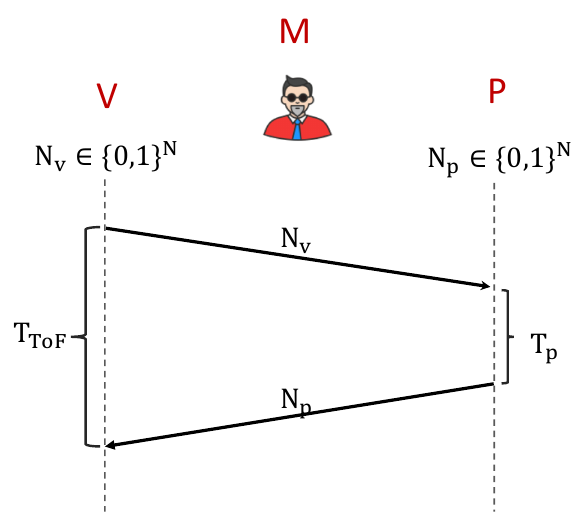
\includegraphics[scale=0.4]{images/5-model.png}
	\caption{Model of the distance bounding scenario}
	\label{fig:ranging-model}
\end{figure}

\paragraph{Types of attacks (frauds)}
\begin{itemize}
	\item \textbf{Distance fraud:} A dishonest $P$ tries to change its distance to $V$.
	\item \textbf{Mafia fraud:} Honest $V, P$ being attacked by an external $M$.
	\item \textbf{Terrorist fraud:} Dishonest $P$ and $M$ collude to change $P$'s distance.
	\item \textbf{Distance hijacking:} Dishonest $P$ leverages an honest $P$ to change its distance.
\end{itemize}

\paragraph{Physical layer: Representing bits as pulses (UWB)}
There are two design options to represent a bit: either with a single strong pulse or a sequence of weaker pulses.
Single pulses may not be detected reliably (distance, interference), so the aggregate over several pulses is the preferred representation.

\begin{figure}
	\centering
	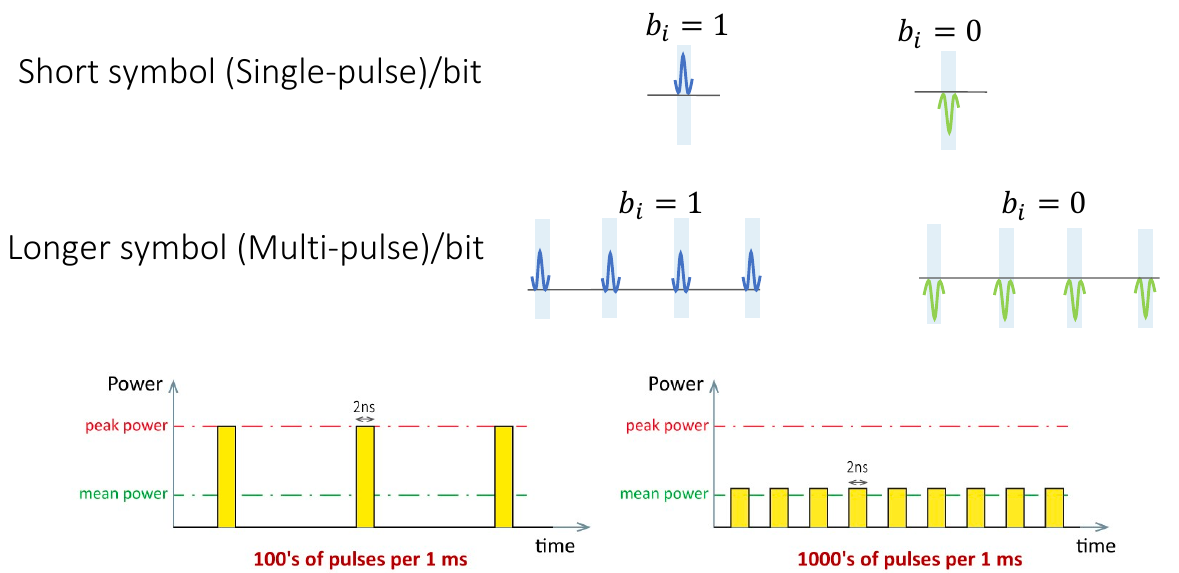
\includegraphics[scale=0.4]{images/5-single-multi-pulse.png}
	\caption{Bit representation: single- versus multi-pulse}
	\label{fig:single-multi-pulse}
\end{figure}

\paragraph{Early-Detect/Late-Commit attack (ED/LC)}
This attacks shortens the distance, since the receiver receives the first symbols earlier than it should have.

\begin{enumerate}
	\item Attacker sends noise (at time $T_A$)
	\item Attacker learns correct symbol (at time $T_{ed}$)
	\item Attacker commits to correct symbol (at time $T_{lc}$), by sending the remaining pulses such that the sum over all pulses matches.
\end{enumerate}

Note that this attack is not possible with single pulses.
A single pulse is usually 1-2 ns long, so the attacker can cheat by at most 15-30 cm (performance/security tradeoff).

\begin{figure}
	\centering
	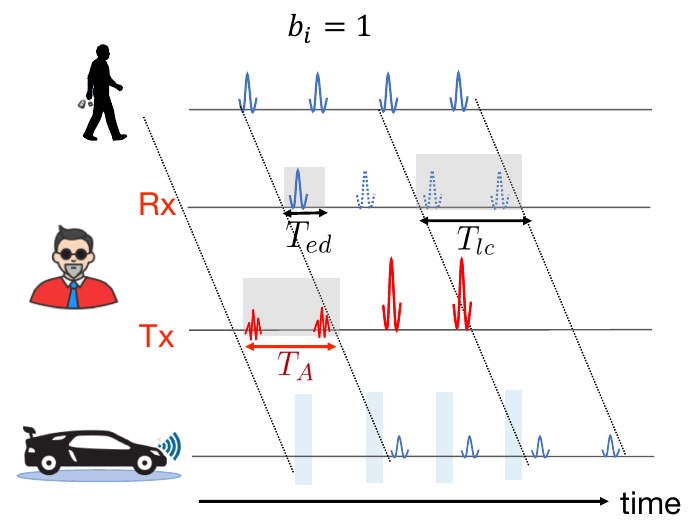
\includegraphics[scale=0.4]{images/5-edlc.png}
	\caption{Early-Detect/Late-Commit attack (ED/LC)}
	\label{fig:edlc}
\end{figure}

\paragraph{ED/LC Solution 1: Pulse Reordering UWB-PR}
Interleave pulses of subsequent symbols according to some cryptographic reordering.
Thus the start and end time of a symbol is unpredictable, and the attacker can only guess.
\\
The probability of an attack decreases [increases] with the number of interleaved bits [number of pulses per bit].

\begin{figure}
	\centering
	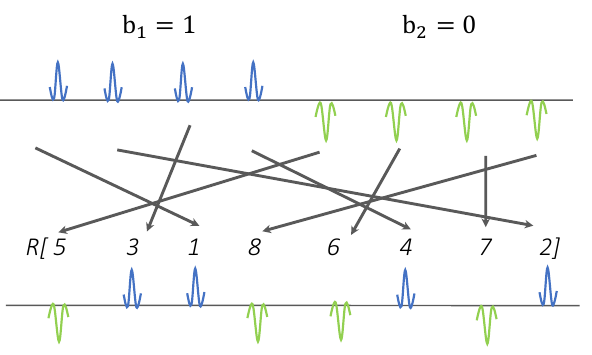
\includegraphics[scale=0.45]{images/5-pulse-reordering.png}
	\caption{Pulse Reordering}
	\label{fig:pulse-reordering}
\end{figure}

\paragraph{ED/LC Solution 2: Variance Based Detection}
Statistically analyse the received versus the expected pulses.
This forces the attacker to ``guess better'' to reduce the variance and make their error indistinguishable from the noise.

\begin{figure}
	\centering
	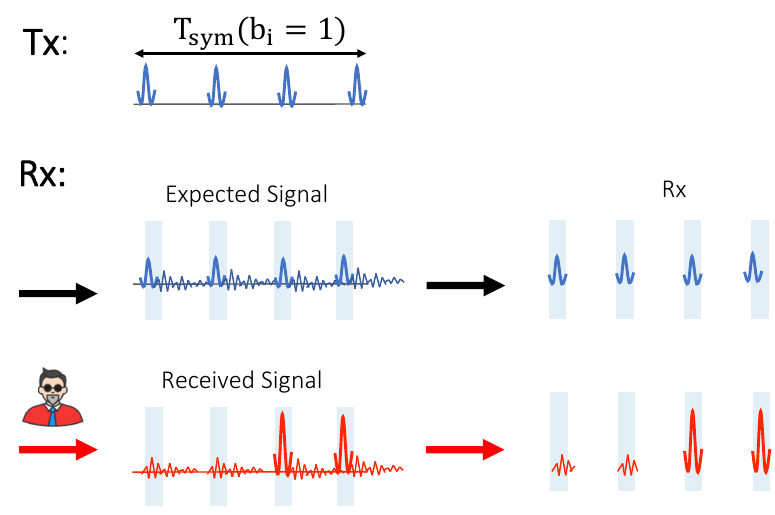
\includegraphics[scale=0.4]{images/5-variance-based.png}
	\caption{Variance Based Detection}
	\label{fig:variance-based}
\end{figure}

\paragraph{ED/LC Solution 3: Scrambled Timestamp Sequence}

After the preamble (high correlation) which is used for ToF \textit{estimation},
send a Scrambled Timestamp Sequence STS (encrypted with a shared secret, low autocorrelation) to use for ToF \textit{verification}.
\\
See IEEE 802.15.4z.
Security not formally proven and unclear!

\begin{figure}
	\centering
	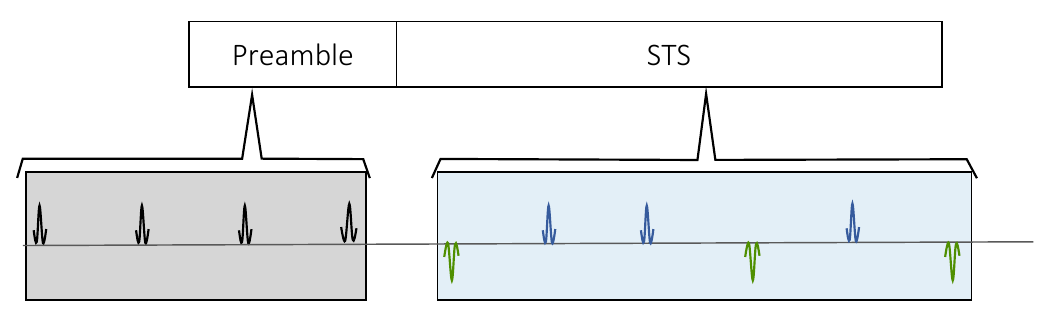
\includegraphics[scale=0.35]{images/5-scrambled-timestamp.png}
	\caption{Scrambled Timestamp Sequence}
	\label{fig:scrambled-timestamp}
\end{figure}

\paragraph{IEEE 802.15.4z LRP versus HRP}
\mbox{}
\begin{table}[h]
\centering
\begin{tabular}{ll}
Low Rate Pulse LRP & High Rate Pulse HRP\\
\hline
Can use single pulse & No single pulse (energy too low) \\
Multi-pulse with UWB-PR efficient & UWB-PR + variance-based seem inefficient \\
Open security specs & No open security analysis \\
Low-cost, low-energy &
\end{tabular}
\end{table}

\paragraph{Message Time of Arrival Code MTAC}
New class of cryptographic primitives that verify the integrity of message arrival time.
E.g.: single-pulse, UWB-PR, Variance-based detection.

\begin{figure}
	\centering
	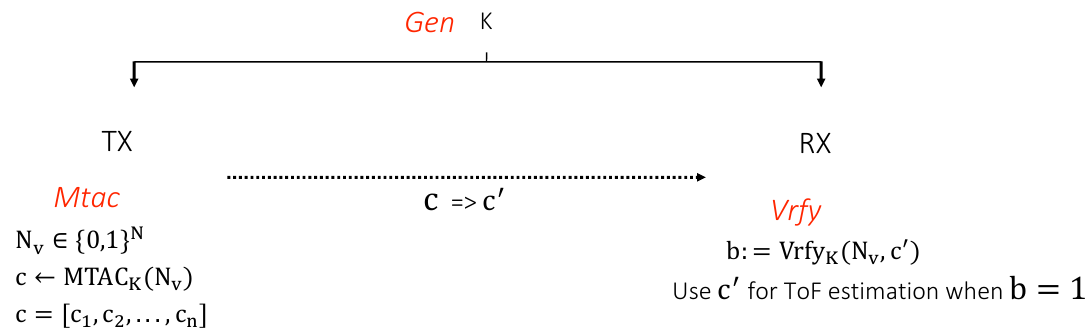
\includegraphics[scale=0.4]{images/5-mtac.png}
	\caption{Message Time of Arrival Code MTAC}
	\label{fig:mtac}
\end{figure}

\paragraph{Verifiable Multilateration}
Multiple verifiers with known locations want to determine the position of a prover.
C.f. GPS trilateration.
E.g. to position autonomous cars using cell towers.

\paragraph{Future Work}
\begin{itemize}
	\item Secure Positioning (e.g. verifiable multilateration)
	\item WiFi 802.11 and 5G ranging (some initial work)
	\item Efficient implementation + deployment
\end{itemize}
